\documentclass[10pt,a4paper]{article}
\usepackage{amssymb,amsmath}
\usepackage{cite}
\usepackage[framed,numbered,autolinebreaks,useliterate]{mcode}
\usepackage[pdftex]{graphicx}
\DeclareGraphicsExtensions{.jpg,.png}
\graphicspath{{images/}}



\begin{document}
\title{Ass5 Solutions}
\author{Chang Li}
\maketitle

\section{Solutions}

\subsection{Linear Programming}
The problem reaches its optimal value when
\begin{align*}
  x=\begin{bmatrix}
    0.5\\
    0.5\\
    0\\
    0
  \end{bmatrix}
\end{align*}
The optimal value is $1.5$.

The following is the source code:
\begin{lstlisting}
  %% Q1: LINEAR PROGRAMMING
  clearvars;
  % Input data
  n = 4;
  % Parameters of objective function
  q = [1,2,3,4];
  % Parameters of equality constraints
  C = [1,1,1,1;1,-1,1,-1];
  d = [1;0];
  % Parameters of inequal constraints
  l = [0,0,0,0]';

  % cvx opt
  cvx_begin
    variable x(n)
    minimize( q*x )
    subject to
    C*x==d
    l<=x
  cvx_end
\end{lstlisting}

\subsection{Regularized Maximum Likelihood Estimation}

\subsubsection{a}
Because dataset $D$ is drawn from a Gaussian distribution
with mean $\mu$ and covariance $\Sigma$. Suppose $x\in R^n$,
so the density is:
$$p(x) = (2\pi)^{-n/2}det(\Sigma)^{-1/2}exp(-(x-\mu)^T\Sigma^{-1}(x-\mu)/2)$$

The average log-likelihood function has the form:
\begin{align*}
  l(D) & = E(\text{log}\;p(x_1,x_2,\dots,x_m))\\
       & = E(-\text{log}\;(2\pi) - \text{log}\;det\Sigma
  - \sum_{i=1}^{M}(-(x_i-\mu)^T\Sigma^{-1}(x_i-\mu)))
\end{align*}
Since $(x-\mu)^T\Sigma^{-1}(x-\mu)$ is a number and
$\mathrm{trace}(AB)=\mathrm{trace}(BA)$ therefore,
$$(x-\mu)^T\Sigma^{-1}(x-\mu)= \mathrm{tr}((x-\mu)^T\Sigma^{-1}(x-\mu))=\mathrm{tr}(\Sigma^{-1}(x-\mu)^T(x-\mu))$$ 
Plugging into expectation we get:
\begin{align*}
E[(x-\mu)^T\Sigma^{-1}(x-\mu)] &= E[\mathrm{tr}((x-\mu)^T(x-\mu)\Sigma^{-1}] )] \\
&= \mathrm{tr}(E[(x-\mu)^T(x-\mu)\Sigma^{-1}])\\
&= \mathrm{tr}(\hat{\Sigma}\Sigma^{-1})
\end{align*}
Plugging into the third term of $l(D)$ we can reformulate it as:
\begin{align*}
     l(D) &=- \text{log}\;det\Sigma - tr(\hat{\Sigma}\Sigma^{-1} )+ const \\
       & = \text{log}\;det\Sigma^{-1} - tr(\hat{\Sigma}\Sigma^{-1} ) + const 
\end{align*}

\subsubsection{b}
Because $K\succ 0$, we use the fact in section
3.1.5\cite{boyd2004convex} that the log of determinant is
concave so its negation is convex and
$\mathrm{tr}(\hat{\Sigma}K)$ is also convex. And the
absolute value function and summation operation are also
convex operations. Therefore the regularized maximum
likelihood optimization problem is a summation of convex
functions and hence the Total Variation Denoising problem is
convex.

\subsubsection{c}
The following figure~\ref{fig:q2vs} uses $\lambda\in [1e-5,10]$ as $x$
axis. The blue line is number of non-zero elements in the
matrix. The red line is the optimal value of the problem.
The yellow line is the corresponding value of log-likelihood
without regularization term.
\begin{figure*}
  \centering
	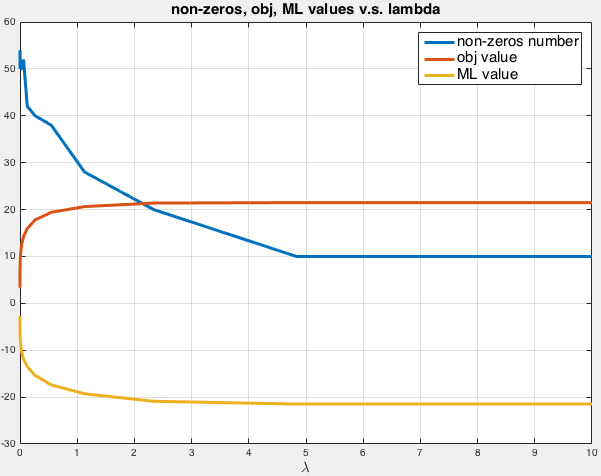
\includegraphics[width=0.7\linewidth]{Q2_vslambda.png}
  \caption{values change versus lambda}
  \label{fig:q2vs}
\end{figure*}

The following is the source code:

\begin{lstlisting}
  %% Q2: Regularized ML Estimation
  clearvars;
  load asgn5q2.mat;
  % Input data
  [m, n] = size(X);
  x_corr = cov(X);
  % off diagonal matrix
  idx = 1-eye(n,n);
  sum_idx = ones(1,n);
  % range of lambda
  iters_num = 20;
  lambda_arr = logspace( -5, 1, iters_num );
  % Results history arrays
  S_nonzeros_arr = zeros(1,iters_num);
  obj_arr = zeros(1,iters_num);
  ml_arr = zeros(1,iters_num);

  % cvx opt loop
  for i=1:iters_num
    lambda = lambda_arr(i);
    cvx_begin sdp
      variable S(n,n) symmetric 
      minimize ( -log_det(S) + trace(x_corr*S)...
      + lambda * sum_idx * abs(idx.*S)*sum_idx' );
      subject to
      S==semidefinite(n,n);
    cvx_end

    % record history
    ml_arr(i) = log_det(S) - trace(x_corr*S);
    obj_arr(i) = cvx_optval;
    S_nonzeros_arr(i) = sum(sum(S>1e-6));
  end

  % plot graph
  figure();
  plot(lambda_arr,[S_nonzeros_arr;obj_arr;ml_arr], 'LineWidth', 3);
  xlabel('\lambda','FontSize',15);
  l = legend('non-zeros number', 'obj value', 'ML value');
  set(l, 'FontSize',15);
  title('non-zeros, obj, ML values v.s. lambda', 'FontSize',15);
  grid on;
\end{lstlisting}

\subsection{Total Variation Denoising}
To find a ``good'' value of $\lambda$, we print out the
trade-off curve between $||D*\hat{x}||_1$ and
$||\hat{x}-x_{corr}||_2$ in the following figure~\ref{fig:q3tradeoff}:

\begin{figure}[ht]
  \centering
  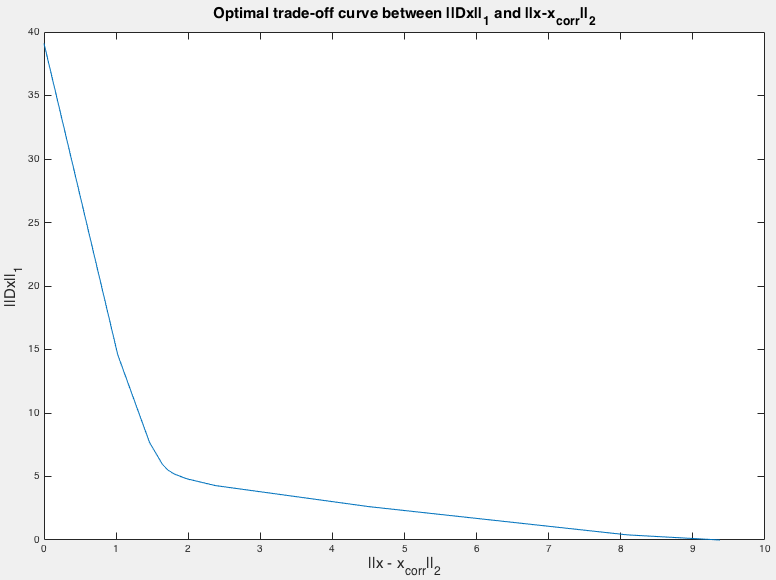
\includegraphics[width=0.7\linewidth]{Q3_tradeoff}
  \caption{trade-off curve}
  \label{fig:q3tradeoff}
\end{figure}

We can find that when $||D*\hat{x}||_1$ is around
$[4.8,5.2]$, the curve has a clear knee. After some
experiments we found when $\lambda = 0.2212$ the recovered
signal has relatively good performance. The following is a
figure~\ref{fig:q3recovered} to show our contrast between the original corrupted
signal and the signal recovered when $\lambda = 0.2212$:


\begin{figure}[ht]
  \centering
  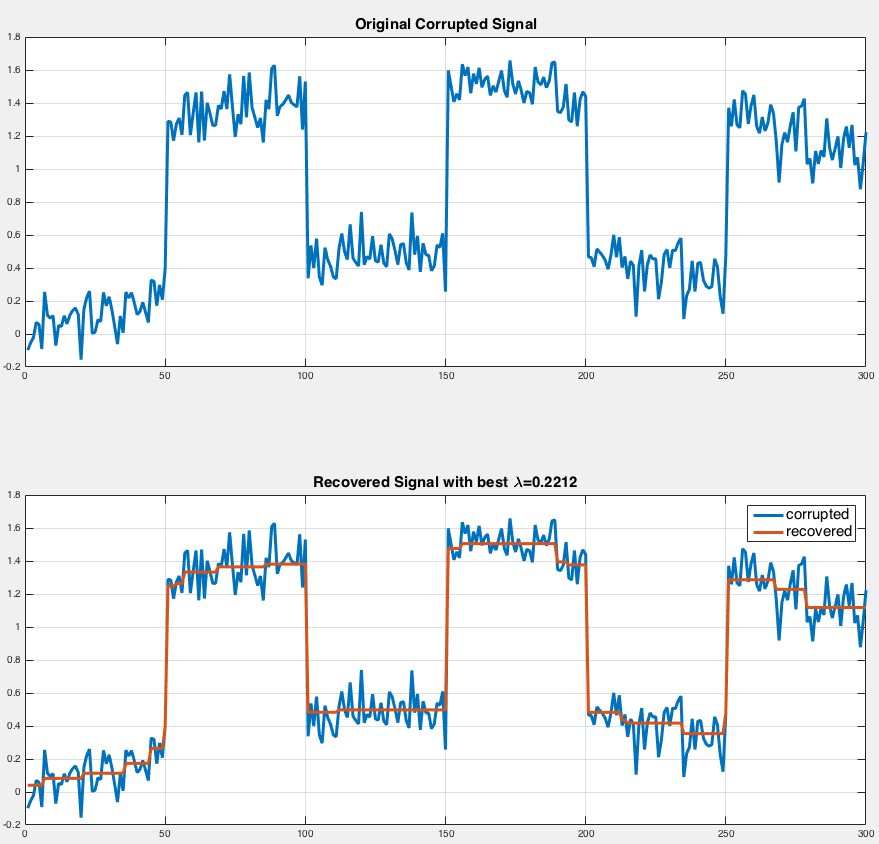
\includegraphics[width=0.8\linewidth]{Q3_signal}
  \caption{original and recovered signal}
  \label{fig:q3recovered}
\end{figure}

In the figure~\ref{fig:q3recovered} we can observe that most of the noisy are
smoothed away, which means the regularize term gives a
significant noisy reduction. However, at the same time the
rapid variations in the original signal are also preserved.
So we think this value is much preferable.


The following is the source code:
\begin{lstlisting}
  %% Q3: Total Variation Denoising
  clearvars;
  load asgn5q3.mat;
  % input data
  n = length(x_corr);
  % difference matrix
  e = ones(n,1);
  D = spdiags([-e e], -1:0, n, n);
  D(1)=0;
  % range of lambda
  iters_num = 30;
  lambda_arr = logspace( -5,1, iters_num );
  % Results history arrays
  obj_arr = zeros(1,iters_num);
  norm_error = zeros(1,iters_num);
  norm_regu = zeros(1,iters_num);

  % cvx opt loop
  for i = 1:iters_num
    lambda = lambda_arr(i);
    cvx_begin
      variable x(n)
      minimize( norm(x-x_corr) + lambda*norm(D*x,1));
    cvx_end
    % record history
    obj_arr(i) = cvx_optval;
    norm_error(i) = norm(x-x_corr);
    norm_regu(i) = norm(D*x,1);
  end

  % plot graph
  figure();
  plot(1:iters_num,[lambda_arr;obj_arr]);
  l_lambda = legend('\lambda','obj value');
  set(l_lambda,'FontSize',15);
  title('obj value v.s. \lambda', 'FontSize',15);
  figure();
  plot(norm_error, norm_regu);
  xlabel('||x - x_{corr}||_2', 'FontSize',15);
  ylabel('||Dx||_1', 'FontSize',15);
  title('Optimal trade-off curve between ||Dx||_1 and ||x-x_{corr}||_2', 'FontSize',15);

  % Best lambda we choose
  lambda=0.2212;
  cvx_begin
  variable x(n)
  minimize( norm(x-x_corr) + lambda*norm(D*x,1));
  cvx_end
  % Plot Recovered Results
  figure();
  subplot(2,1,1);
  plot(1:n, x_corr, 'LineWidth', 3);
  grid on;
  title('Original Corrupted Signal','FontSize', 15);
  subplot(2,1,2);
  plot(1:n, [x_corr';x'], 'LineWidth', 3);
  l = legend('corrupted', 'recovered');
  set(l,'FontSize',15);
  grid on;
  title('Recovered Signal with best \lambda=0.2212','FontSize',15);
\end{lstlisting}

	\renewcommand\refname{Bibliography}
	\bibliographystyle{ieeetr}
	\bibliography{ass5_ChangLi}
\end{document}
